\documentclass[letterpaper, landscape]{exam}
\usepackage{2in1, lscape} 
\printanswers

\usepackage{units} 
\usepackage[fleqn]{amsmath}
\usepackage{float}
\usepackage{mdwlist}
\usepackage{booktabs}
\usepackage{caption}
\usepackage{fullpage}
\usepackage{enumerate}
\usepackage{graphicx}
\usepackage[justification=justified]{caption}

\setcounter{tocdepth}{1}
\everymath{\displaystyle}

\author{}
\date{\today}
\title{Calculus I \\ Week Eight}

\begin{document}

  \maketitle
  \tableofcontents

  \section{Homework 2.5}

  Homework 2.5, problem 62: 
  \begin{solution}
    \begin{align*}
      \lim_{x \to 1^-} f(x) &= - \infty \\ 
      \lim_{x \to -1^+} f(x) &= \infty \\ 
    \end{align*}

    Since there are always values of $x$ where $f(x) < 0-$ and values of
    $x$ where $f(x) > 0$ in the interval $(-1, 1)$, and $f$ is continuous on $(1, 1)$,
    there is some value of $x$ where $f(x) = 0$ in the same interval.

  \end{solution}

  Talk about Homework 2.4, problem 43

  \section{Derivative as a Function}

  \begin{itemize*}
    \item Show formula for derivative as a function.
    \item Show graphs of derivatives
    \item Show graphs of derivatives where $f(x)$ is sequence of line segments
    \item Show graphs of polynomial derivatives (see below)
    \item Show graph of $f(x) = e^x$
  \end{itemize*}

  \begin{figure}[H]
    \centering
    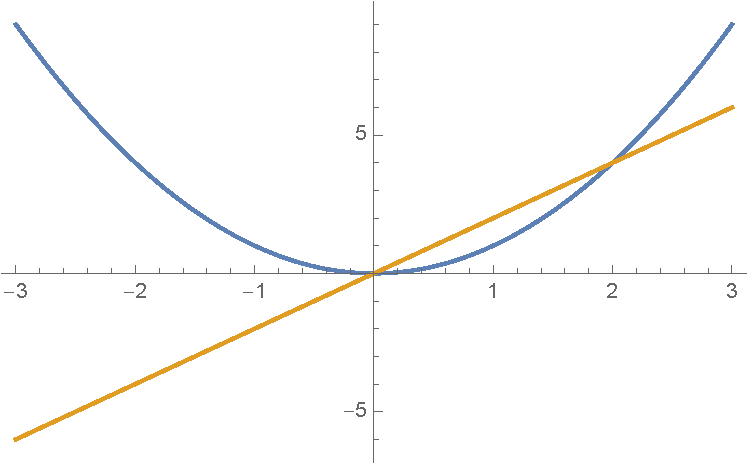
\includegraphics[scale = 0.5]{example06.pdf}
    \caption{$f(x) = x^2$}
    \label{fig:example06}
  \end{figure}

  \begin{figure}[H]
    \centering
    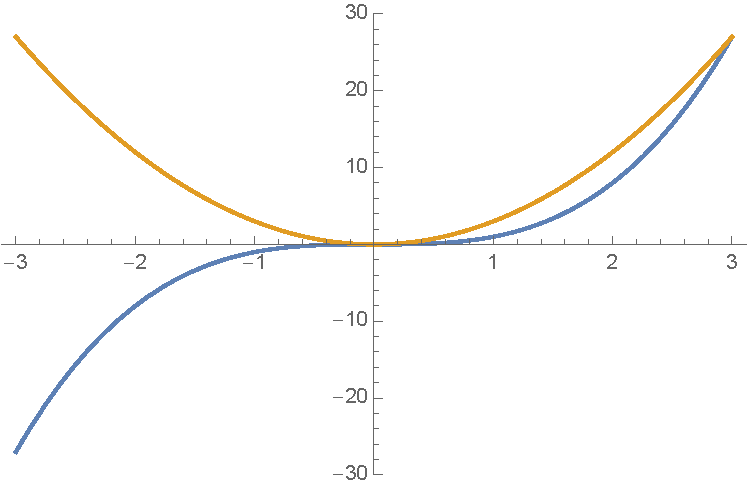
\includegraphics[scale = 0.5]{example03.pdf}
    \caption{$f(x) = x^3$}
    \label{fig:example03}
  \end{figure}

  \begin{figure}[H]
    \centering
    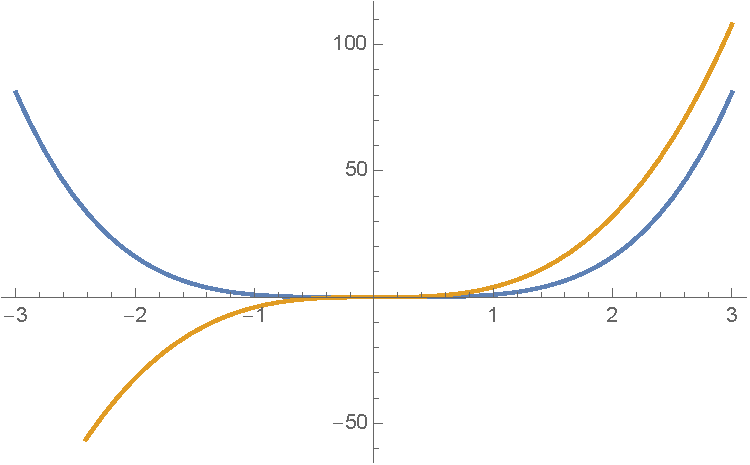
\includegraphics[scale = 0.5]{example04.pdf}
    \caption{$f(x) = x^4$}
    \label{fig:example04}
  \end{figure}

  \begin{figure}[H]
    \centering
    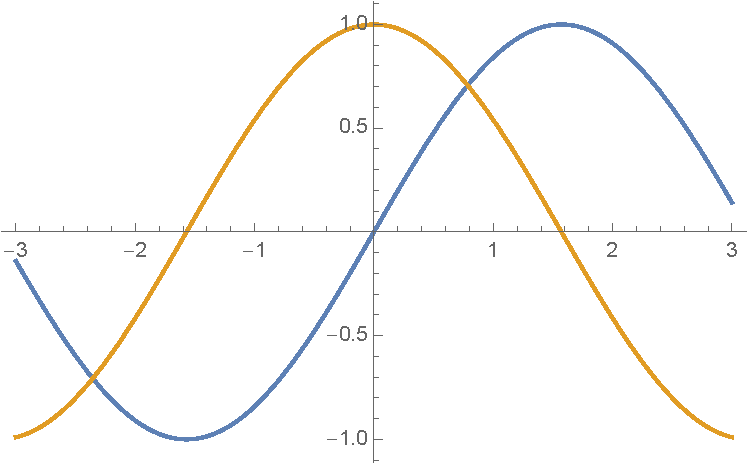
\includegraphics[scale = 0.5]{example05.pdf}
    \caption{$f(x) = \sin(x)$}
    \label{fig:example05}
  \end{figure}

  \begin{figure}[H]
    \centering
    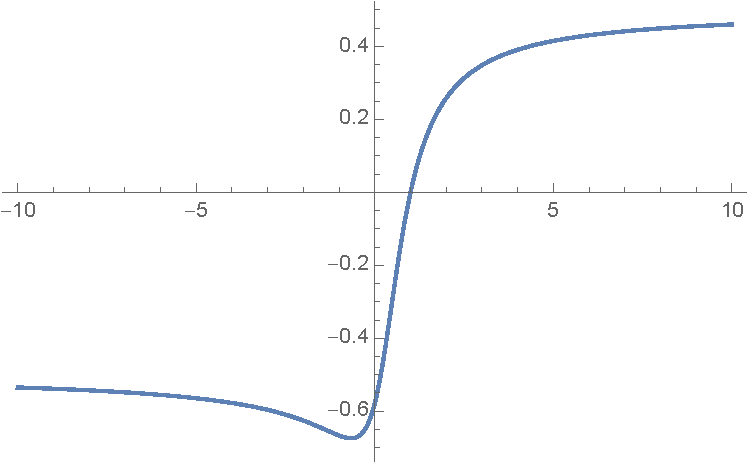
\includegraphics[scale = 0.5]{example01.pdf}
    \caption{Third Degree Polynomial}
    \label{fig:example01}
  \end{figure}

  \begin{figure}[H]
    \centering
    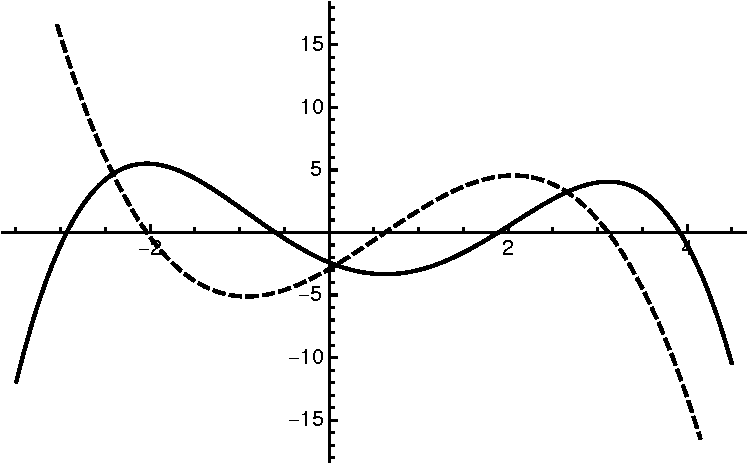
\includegraphics[scale = 0.5]{example02.pdf}
    \caption{Fourth Degree Polynomial}
    \label{fig:example02}
  \end{figure}

  \section{Derivative Examples}

  \begin{enumerate}
    \item 
      \[
        f(x) = 3x^2 + x
      \]
    \item 
      \[
        f(x) = x^3 - 2x^2 + x + 1
      \]

    \item 
      \[
        f(x) = \frac{1}{\sqrt{x}}
      \]

      \begin{solution}
        \[
          f'(x) = \frac{-1}{2 x^{3/2}}
        \]
      \end{solution}

    \item 
      \[
        f(x) = \sqrt{x^2 + 1}
      \]

      \begin{solution}
        \[
          f'(x) = \frac{x}{\sqrt{x^2 + 1}}
        \]
      \end{solution}

    \item 
      \[
        f(x) = \frac{2x + 1}{x - 1}
      \]

      \begin{solution}
        \[
          f'(x) = \frac{-3}{(x - 1)^2}
        \]
      \end{solution}

  \end{enumerate}

  \section{Differentiability}

  \begin{itemize}
    \item $f$ is differentiable on $(a, b)$ if $f'$ is defined on $(a, b)$
    \item show graph of corners where $\lim_{x \to a^-} \neq \lim_{x \to a^+}$
    \item $f(x) = |x|$ is not differentiable at $x = 0$
  \end{itemize}

  \section{Continuity}
  If $f$ is differentiable at $a$ then $f$ is continuous at $a$ (not necessarily
  vice-versa).

  proof: show that if $\lim{h \to 0} \frac{f(x + h) - f(x)}{h}$ is defined then
  $\lim{h \to 0} f(x + h) = f(x)$ (variation on proof in book)

  \begin{align*}
    f(x + h) - f(x)                               & = \frac{f(x + h) - f(x)}{h} \cdot h \\
    \lim_{h \to 0} \left[ f(x + h) - f(x) \right] & = \lim_{h \to 0} \left[  \frac{f(x + h) - f(x)}{h} \cdot h \right] \\
    \lim_{h \to 0} f(x + h) - \lim_{h \to 0} f(x) & =  f'(x) \cdot \lim_{h \to 0} h  \\
    \lim_{h \to 0} f(x + h) - \lim_{h \to 0} f(x) & =  0 \\
    \lim_{h \to 0} f(x + h)                       & = \lim_{h \to 0} f(x) \\
    \lim_{h \to 0} f(x + h)                       & = f(x) \\
  \end{align*}

  \section{Second Derivatives}


  Calculate first and second derivatives of ball thrown from height 5 meters (approximate):
  \[
    h(t) = 5 + 30t - 5t^2
  \]

  \begin{figure}[H]
    \centering
    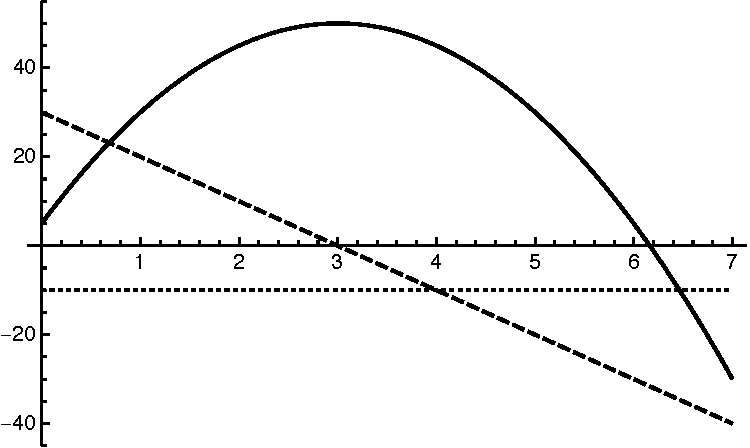
\includegraphics[scale = 0.5]{example07.pdf}
    \caption{Height, Velocity, and Acceleration}
    \label{fig:example07}
  \end{figure}

\end{document}

